\documentclass[aps,showpacs,twocolumn,prd,superscriptaddress,nofootinbib]{revtex4-1}

\usepackage{amsmath}
\usepackage{amsfonts}
\usepackage{amssymb}
\usepackage{latexsym}
\usepackage{graphicx}
\usepackage{bm}
%\usepackage{color}
\usepackage{enumerate}
\usepackage{ulem}
\usepackage{tabularx}
\usepackage{braket}

\usepackage{color}
\usepackage[usenames,dvipsnames,svgnames,table]{xcolor}
%\usepackage[colorlinks=true,
%            linkcolor=green,
%            urlcolor=blue,
%            citecolor=red]{hyperref}
\usepackage[colorlinks=true,
            linkcolor=YellowOrange,
            urlcolor=RoyalBlue,
            citecolor=RedViolet]{hyperref}

\newcommand{\be}{\begin{equation}}
\newcommand{\ee}{\end{equation}}
\newcommand{\bsub}{\begin{subequations}}
\newcommand{\esub}{\end{subequations}}
\newcommand\ud{{\mathrm{d}}}
\newcommand\uD{{\mathrm{D}}}
\newcommand\calO{{\mathcal{O}}}
\newcommand\calM{{\mathcal{M}}}
\newcommand\calF{{\mathcal{F}}}
\newcommand\calT{{\mathcal{T}}}
\newcommand\calD{{\mathcal{D}}}
\newcommand\calA{{\mathcal{A}}}
\newcommand\calL{{\mathcal{L}}}
\newcommand\bfx{\mathbf{x}}
\newcommand{\ov}[1]{\overline{#1}}
\newcommand{\ph}[1]{\phantom{#1}}
\newcommand{\cte}{\mathrm{cte}}
\newcommand{\nn}{\nonumber}
\newcommand{\hatk}{\hat{k}}
\newcommand{\Hz}{\,\mathrm{Hz}}
\newcommand{\sinc}{\,\mathrm{sinc}}
\newcommand{\Msol}{M_{\odot}}
\newcommand{\Mchirp}{M_{c}}
\newcommand\betaL{{\beta_{L}}}
\newcommand\lambdaL{{\lambda_{L}}}
\newcommand\varphiL{{\varphi_{L}}}
\newcommand\psiL{{\psi_{L}}}
\newcommand{\tf}{t_{f}}
\newcommand{\Tf}{T_{f}}
\newcommand{\tfd}{t_{f}^{d}}
\newcommand{\tfSPA}{t_{f}^{\rm SPA}}
\newcommand{\TfSPA}{T_{f}^{\rm SPA}}
\newcommand{\sYlm}{{}_{-2}Y_{\ell m}}
\newcommand{\sYlmstar}{{}_{-2}Y_{\ell m}^{*}}
\newcommand{\sYlminusmstar}{{}_{-2}Y_{\ell, -m}^{*}}

\newcolumntype{C}[1]{>{\centering\arraybackslash}p{#1}}
\newcolumntype{L}[1]{>{\raggedright\arraybackslash}p{#1}}

\newcommand{\SM}[1]{{\color{Blue} #1}}
\newcommand{\jgb}[1]{{\color{DarkGreen} #1}}
\newcommand{\tdc}[1]{{\color{red} #1}}

\begin{document}

\title{Bayesian methods for black hole merger parameter estimation with LISA.}

\author{John G. Baker}
\affiliation{Gravitational Astrophysics Laboratory, NASA Goddard Space Flight Center, 8800 Greenbelt Rd., Greenbelt, MD 20771, USA}
\author{Sylvain Marsat}
\affiliation{APC, AstroParticule et Cosmologie, Universit\'{e} Paris Diderot, CNRS/IN2P3, CEA/Irfu, Observatoire de Paris, Sorbonne Paris Cit\'{e}, 10, rue Alice Domon et L\'{e}onie Duquet 75205 PARIS Cedex 13, France}
\author{Tito Dal Canton}
\affiliation{Gravitational Astrophysics Laboratory, NASA Goddard Space Flight Center, 8800 Greenbelt Rd., Greenbelt, MD 20771, USA}


\date{\today}

\begin{abstract}

[Abstract]

\end{abstract}

\pacs{
04.70.Bw, % classical black holes
04.80.Nn, % Gravitational wave detectors and experiments
95.30.Sf, % relativity and gravitation
95.55.Ym, % Gravitational radiation detectors
97.60.Lf  % black holes (astrophysics)
}

\maketitle

%%%%%%%%%%%%%%%%%%%%%%%%%%%%%%%%%%%%
%%%%%%%%%%%%%%%%%%%%%%%%%%%%%%%%%%%%

\section{Introduction}
\label{sec:intro}

[Introduction]

%%%%%%%%%%%%%%%%%%%%%%%%%%%%%%%%%%%%
%%%%%%%%%%%%%%%%%%%%%%%%%%%%%%%%%%%%

\section{The LISA instrument response}
\label{sec:response}

%%%%%%%%%%%%%%%%%%%%%%%%%%%%%%%%%%%%

\subsection{The LISA response - OLD}
\label{sec:lisaresponse}

\SM{------------------------------------------------------}

\SM{[copy-paste from previous paper -- just here to copy needed formulas / refs]}

We begin by detailing the model that we use for the response of a LISA-like detector, together with the assumptions used and their limitations. Since our aim is to assess the accuracy of our direct Fourier-domain treatment of the response, we can focus on the gravitational-wave contribution to the basic single-link observables. We therefore use a somewhat simplified model for the time-domain response~\cite{Krolak+04}, ignoring corrections that would be crucial from the point of view of noise cancellations, keeping in mind that the response model can be enriched later without affecting the conclusions of the present analysis.

The frequency-shift response for a single link~\eqref{eq:yslr} was derived in Ref.~\cite{EW75} (see also~\cite{CR02, RCP04, Finn08, Cornish09}). Several assumptions enter the result as written in~\eqref{eq:yslr}: (i) effects of the order $v/c$ are neglected, including for instance the special relativistic Doppler effect created by the relative speeds of the spacecraft on their orbits (ii) the propagation is assumed to take place in a flat spacetime, perturbed only by the gravitational wave; thus the gravitational redshift as well as the deflection of light created by the gravitational potential of the Sun is ignored (iii) all geometric factors are evaluated at a single time, whereas one should consider the beam as propagating from the position of the first spacecraft at the time of emission to the position of the second scapecraft at the time of reception, leading to a point-ahead effect.

Additionally, we limit ourselves to a rigid model for the orbits of the constellation, namely we assume that the constellation remains in an equilateral configuration with fixed armlengths. These simplified orbits neglect (iv) effects of order $e^{2}$ from the eccentricity of the individual Keplerian orbits, (v) the effect of gravitational perturbations coming from other celestial bodies, such as the Earth, the quadrupole of the Sun, and the other planets. Note that although we can neglect all the effects (i)-(v) for our present study, keeping track of these corrections is crucial for the purpose of laser noise cancellations, and led to the development of new generations of TDI observables~\cite{Tintoliving}.

It is natural to split the response~\eqref{eq:yslr} into two steps: first the orbital delay related to the orbit around the Sun of the whole constellation, and then the constellation response. The baselines for the delays are indeed very different in the two cases. Geometrical projection factors aside, we have for the orbit around the Sun $R=1\text{au}=1.5\times 10^{8} \text{km}$, while the detector armlength is $L=2.5\times 10^{6}\text{km}$ (in the configuration proposed in~\cite{LISA17}). It is natural to define two transfer frequencies for the two relevant length scales for the delays, defined such that a wavelength fits within this length scale, i.e. $2\pi f d = 1$. This gives
\begin{subequations}\label{eq:transferfrequencies}
\begin{align}
	f_{R} &= 3.2\times10^{-4}\Hz \,,\\
	f_{L} &= 1.9\times 10^{-2}\Hz \,.
\end{align}
\end{subequations}
The LISA response will behave qualitatively differently on the three frequency bands $f \leq f_{R}$, $f_{R} \leq f \leq f_{L}$ and $f_{L} \leq f$.

The first stage of the response, the orbital delay, consists simply in applying the varying time delay to bring the wavefront sampling point from the SSB reference to the center of the LISA triangular constellation, common to all $y_{slr}$ observables. For $h^{\rm TT}$ the transverse-traceless gravitational waveform in matrix form, we write this orbital time delay as
\be\label{eq:defresponse0}
	h_{0}^{\rm TT} (t) = h^{\rm TT}(t-\hatk\cdot p_{0}) \,,
\ee
with $p_{0}$ the position of the constellation center, which follows the Earth orbit around the Sun. The second stage of the response calculation comprises the remaining, constellation-centered response. For the single-link contribution to the response, for the laser link from spacecraft $s$ to spacecraft $r$ along a path in direction $n_l$, we write
\begin{align}\label{eq:defresponseL}
	y_{slr} &= \frac{1}{2} \frac{1}{1 - \hatk\cdot n_{l}} \nn\\
	& \cdot n_{l}\cdot \left[ h_{0}^{\rm TT}(t - L - \hatk\cdot p^{L}_{s}) - h_{0}^{\rm TT}(t - \hatk\cdot p^{L}_{r}) \right] \cdot n_{l}\,,
\end{align}
where we reference the positions of the spacecraft relative to the center of the constellation, $p^{L}_{A} \equiv p_{A} - p_{0}$.

As described in App.~\ref{app:notation} We will decompose the full signal in the contributions of the individual spin-weighted spherical modes $h_{\ell m}$, whose Fourier transforms are assumed to have a smooth amplitude and phase. First, we define the matrices $P_{+},P_{\times}$ such that, in the sense of matrices,
\be
	h^{\rm TT} = h_{+}P_{+} + h_{\times}P_{\times} \,.
\ee
We focus only on positive frequencies. Assuming that the approximation~\eqref{eq:zeronegativef} applies, we consider a single mode contribution, $h=h_{\ell m}$ with $m>0$. For each given mode we define a complex matrix $P_{\ell m}$ incorporating the spin-weighted spherical harmonic constant factor as
\be
	P_{\ell m} =
	\begin{cases}
	\frac{1}{2} {}_{-2}Y_{\ell m} \left( P_{+} + i P_{\times} \right) \text{ for } m>0\,,\\
	\frac{1}{2} {}_{-2}Y_{\ell m}^{*} \left( P_{+} - i P_{\times} \right) \text{ for } m<0\,.
	\end{cases}
\ee

We now turn to the transformation of~\eqref{eq:defresponse0} and~\eqref{eq:defresponseL} to the Fourier domain. Applying a pure delay as in~\eqref{eq:defresponse0} translates into
\be\label{eq:G0}
	G_{0}(f, t) = e^{-2i\pi f d_{0}(t)} \,,
\ee
with $d_{0} = -\hatk \cdot p_{0}$ the delay associated to the orbit around the Sun. For the leading-order response~\eqref{eq:transferlocal}, this gives a Fourier-domain transfer function common to all modes, that is a pure phase factor, proportional to the frequency but also $t_{f}$-dependent:
\be\label{eq:transfer0local}
	\calT_{0}^{\rm local}(f) = G_{0}(f, \tf)\,.
\ee
If $(\lambda, \beta)$ are the ecliptic longitude and latitude of the source in the sky, and if the orbital phase is set by convention to $0$ at $t=0$, the orbital delay has the simple expression
\be\label{eq:delay0}
	d_{0}(t) = -R \cos\beta \cos\left(\Omega_{0}t - \lambda\right)\,.
\ee

For the constellation part of response~\eqref{eq:defresponseL}, treated separately from the delay~\eqref{eq:delay0}, we write
\begin{align}\label{eq:decomposeGslr}
	F_{slr}^{L}(t) &= \frac{1}{2} \frac{1}{1 - \hatk\cdot n_{l}(t)} n_{l}(t) \cdot P_{\ell m} \cdot n_{l} (t) \,,\nn\\
	d_{s}(t) &= - k\cdot p_{s}^{L}(t) \,, \quad d_{r}(t) = - k\cdot p_{r}^{L}(t) \,,\nn\\
	G_{slr}^{L}(f,t) &=  F_{slr}^{L}(t) \left( e^{-2i\pi f (d_{s,L}(t) + L)} - e^{-2i\pi f d_{r}(t)} \right) \,.
\end{align}
The superscript $L$ indicates that the orbital delay~\eqref{eq:delay0} is not included. Since we also assume the rigid approximation for the constellation, where the armlengths are fixed, a particular simplification occurs when combining these individual delays, thanks to the relation $p^{L}_{r} - p^{L}_{s} =  L n_{l}$:
\begin{align}\label{eq:GslrL}
	G_{slr}^{L}(f,t) &= \frac{i \pi f L}{2} \sinc \left[ \pi f L\left(1-\hatk\cdot n_{l} \right) \right] \nn\\
	& \quad \cdot \exp\left[ i \pi f \left( L + \hatk\cdot \left( p_{1}^{L} + p_{2}^{L} \right) \right) \right]  n_{l} \cdot P_{\ell m} \cdot n_{l} \,,
\end{align}
with all time-dependent vectors evaluated at $t$. This expression is well known as describing the frequency-dependency in the LISA response~\cite{Larson+99, Cornish01, CR02, RCP04}. In the local approximation~\eqref{eq:transferlocal}, the Fourier-domain transfer function then reads
\begin{align}\label{eq:transferLlocal}
	\calT_{slr}^{L, \mathrm{local}}(f) &= G_{slr}^{L}(f, \tf) \,.
\end{align}
For plotting purposes, we will also define
\be\label{eq:transferLenvelope}
	\overline{\calT}_{slr}^{L} (f) = \frac{i \pi f L}{2} n_{l} \cdot P_{\ell m} \cdot n_{l} (\tf)
\ee
which will serve as an estimate for the enveloppe function of the response, devoid of the zero-crossings at high frequencies of the $\sinc$ term in~\eqref{eq:GslrL}.

Note that, if the corrections of Sec.~\ref{subsec:delays}, for non-negligible $\dot d$, are included for the constellation delays, the transfer function will not have this simple form anymore, as $\dot{d}$ will have a different velocity-dependent expression for the sending and receiving spacecraft. One must then separately handle $d_{s}$ and $d_{r}$ in~\eqref{eq:decomposeGslr} to compute the corrections.

The orbital response~\eqref{eq:transfer0local}-\eqref{eq:delay0} takes a simple analytic form, but the phase contribution of this delay is significant across most of the frequency band and can be large for $f \gg f_{R}$.

The constellation response~\eqref{eq:GslrL}-\eqref{eq:transferLlocal} can be interpreted as the Fourier-domain translation of a discrete derivative taken on the waveform. The leading factor in~\eqref{eq:GslrL} shows that the amplitude of the response is proportional to $f$ in the low-frequency limit $f\ll f_{L}$, where the other factors are essentially unity. For $f\gtrsim f_{L}$, the $\sinc$ and the phase of the exponential generate additional structure in the response, including zero-crossings when the projected armlength is an integer number of wavelengths. From~\eqref{eq:transferLlocal}, an expansion for small $f\ll f_{L}$ yields back a Fourier-domain analog of the low-frequency approximation of the response~\cite{Cutler97, RCP04}, which is equivalent to having two LIGO-type interferometers turned by $\pi/4$ and set in motion.

For analysis of the response we need a concrete set of gravitational waveforms. We will use the PhenomD model~\cite{Khan+15,Husa+15}, which provides Fourier-domain inspiral-merger-ringdown waveforms for aligned spins. We refer to App.~\ref{app:precLISA} for a brief discussion of the prospects for applying our formalism for the LISA response to precessing Fourier-domain waveforms.

\SM{------------------------------------------------------}

%%%%%%%%%%%%%%%%%%%%%%%%%%%%%%%%%%%%

\subsection{The GW signal}
\label{sec:gwsignal}

We start by introducing a source-frame $(\hat{x}_{S}, \hat{y}_{S}, \hat{z}_{S})$ attached to the binary system emitting gravitational waves. For comparable-mass systems without spin, the natural choice is to take the normal to the orbital plane as $\hat{z}_{S}$, and we will assume that the remaining rotation around $\hat{z}_{S}$ is fixed by the phase convention of the waveform model (see Sec.~\ref{}).

Introducing $k$ the wave propagation vector going from the source towards the observer, we define the inclination $\iota$ and the observer phase $\varphi$ simply as being its spherical angular coordinates $(\theta_{S}, \phi_{S})$, so that in the source-frame
\be
	k_{S} = (\sin\iota \cos\varphi, \sin\iota \sin\varphi, \cos\iota) \,.
\ee

By convention, for our polarization vectors $p$ and $q$ we will use the spherical coordinate vectors $p = e_{\theta}^{S}$, $q = e_{\phi}^{S}$. In terms of only $\hat{z}_{S}$,
\bsub
\begin{align}
	p &= q \times k \,,\\
	q &= \hat{z}_{S} \times k / |\hat{z}_{S} \times k|\,.
\end{align}
\esub
If $H_{ij} = h_{ij}^{\rm TT}$ represents the gravitational wave signal in the transverse-traceless gauge,
\be
	H = h_{+} P_{+} + h_{\times} P_{\times}
\ee
with the polarization tensors
\bsub
\begin{align}
	P_{+} &= p \otimes p - q \otimes q \,,\\
	P_{\times} &= p \otimes q + q \otimes p \,.
\end{align}
\esub
Conversely, the polarizations are
\bsub
\begin{align}
	h_{+} &= \frac{1}{2} \left(p \otimes p - q \otimes q \right) : H \,,\\
	h_{\times} &= \frac{1}{2} \left( p \otimes q + q \otimes p \right) : H \,.
\end{align}
\esub

We will further decompose the gravitational wave signal, seen as a function of the direction of emission $(\iota, \varphi)$, in spin-weighted spherical harmonics as
\be\label{eq:hpcmodes}
	h_{+} - i h_{\times} = \sum_{\ell \geq 2} \sum_{m = -\ell}^{\ell} {}_{-2}Y_{\ell m} (\iota, \varphi) h_{\ell m} \,,
\ee
where the explicit expression of the ${}_{-2}Y_{\ell m}$ is given in~\cite{}.

The vectors $(p,q,k)$ form the Wave-frame, such that the gravitational wave takes in this frame the familiar form
\be
	H_{W} = \begin{pmatrix}
		h_{+} & h_{\times} & 0 \\
		h_{\times} & -h_{+} & 0 \\
		0 & 0 & 0
		\end{pmatrix} \,.
\ee

We will both generate the waveforms and apply the response directly in the Fourier domain. Our convention for the Fourier transform is
\be\label{eq:defFourier}
	\tilde{F}(f) = \int dt \; e^{2 i \pi f t} F(t) \,.
\ee
Note that this differs by a change $f\rightarrow -f$ from the most usual one (used e.g. in \texttt{LAL}).

The definition of the reference time and phase \dots

%%%%%%%%%%%%%%%%%%%%%%%%%%%%%%%%%%%%

\subsection{LISA trajectories}
\label{sec:lisatraj}

For completeness, we gather in this appendix explicit expressions for the trajectory of the LISA constellation and the rotation matrices entering the response.

The orbits of the three spacecrafts around the Sun can be chosen so that, at leading order in the eccentricity of the orbits, the constellation retains the shape of an equilateral triangle in a cartwheeling motion following the Earth orbit. We denote by $a$ the semi-major axis, $e$ the eccentricity and pose $\alpha = \Omega_{0} (t-t_{0}))$, with $t_{0}$ a reference time for the initial position ($t_{0} = 0$ in our case). The reference SSB frame is $(\hat{x}, \hat{y}, \hat{z})$.

Using the notation $c,s = \cos, \sin \alpha$, the trajectory of the center of the constellation is simply
\be
	p_{0} = ac \hat{x} + as \hat{y} \,,
\ee
and we take $a\equiv R = 1 \, \mathrm{au}$. We denote the positions of the spacecrafts as $p_{A}$ for $A=1,2,3$, and the positions relative to the constellation center as $p_{A}^{L} = p_{A} - p_{0}$. Setting $\beta_{A} = 2(A-1)\pi/3 + \beta_{0}$ (with $\beta_{0}$ and initial condition set to 0 in our case), the Cartesian coordinates in the SSB-frame of the position of the spacecrafts read~\cite{}
\bsub
\begin{align}
	p_{A}^{L} &= a e \left[ \sin \beta_{A} c s - \cos\beta_{A} \left( 1 + s^{2} \right) \right] \hat{x} \nn\\
	& + a e \left[ \cos \beta_{A} c s - \sin\beta_{A} \left( 1 + c^{2} \right) \right] \hat{y} \nn\\
	& - a e \sqrt{3} \cos(\alpha - \beta_{A}) \hat{z} \,,
\end{align}
\esub
The armlength, constant in this approximation, is related to the eccentricity and semi-major axis by
\be
	L = 2\sqrt{3} a e \,.
\ee
The rigid approximation for the constellation, at first order in $e$, can be seen as being at first order in $L/R \simeq 0.017$ for a $2.5 \, \mathrm{Gm}$ armlength~\cite{}.

%%%%%%%%%%%%%%%%%%%%%%%%%%%%%%%%%%%%

\subsection{The LISA frame}
\label{sec:LISAframe}

It will be very useful to introduce a time-dependent frame $(\hat{x}_{L}, \hat{y}_{L}, \hat{z}_{L})(t)$ following the detector in its motion. Specifically, we choose this LISA frame such that at any time,
\bsub
\begin{align}
	p_{1}^{L} &= - \frac{L}{\sqrt{3}} \hat{x}_{L} \,,\\
	p_{2}^{L} &= \frac{L}{2\sqrt{3}} \hat{x}_{L} - \frac{L}{2} \hat{y}_{L} \,,\\
	p_{3}^{L} &= \frac{L}{2\sqrt{3}} \hat{x}_{L} + \frac{L}{2} \hat{y}_{L} \,.\\
\end{align}
\esub

This frame also provides us with an equivalent representation of the trajectories making use of rotation matrices. Since in our rigid approximation the constellation remains an equilateral triangle in its cartwheeling motion around the Sun, the configuration of the constellation at a later time is given by a rotation around the Sun composed with a rotation of the constellation around its symmetry axis.

If $R(v,\varpi)$ denotes the matrix of an active rotation around the vector $v$ by an angle $\varpi$, and if we denote by $R_{L}$ the active rotation from the SSB-frame to the L-frame such that for each of the three basis vectors $(\hat{x}_{L}, \hat{y}_{L}, \hat{z}_{L}) = R_{L} (\hat{x}, \hat{y}, \hat{z})$, we have
\be\label{eq:RL}
	R_{L} = R(z, \alpha) \cdot R(y, -\pi/3) \cdot R(z, -\alpha) \,,
\ee
where we recall that $\alpha = \Omega_{0} (t-t_{0}) $. For all vectors $X$ among $p_{A}^{L}$, $n_{A}$ we have $X(t) = R_{L} \cdot X(t=t_{0})$. If a vector $X$ is given by its components in the SSB-frame, in the L-frame the components are $X_{L} = R_{L}^{-1} \cdot X$.

%%%%%%%%%%%%%%%%%%%%%%%%%%%%%%%%%%%%

\subsection{From the Wave frame to the SSB frame}
\label{sec:wavessbframe}

We can now relate the Wave-frame to the SSB-frame, which will fix our convention for the sky position and polarization angle. The source position in the sky is given by $(\lambda, \beta)$, the ecliptic longitude and latitude in the SSB-frame. Like with the Source-frame, we can introduce spherical vectors $(e_{r}^{SSB}, e_{\theta}^{SSB}, e_{\phi}^{SSB})$. Since the propagation vector is $k = - e_{r}^{SSB}$,
\be
	k = (- \cos\beta\cos\lambda, - \cos\beta\sin\lambda, -\sin\beta) \,.
\ee

The last degree of freedom between the frames represents a rotation along the line-of-sight, parametrized by the polarization angle $\psi$. We introduce reference polarization vectors in the SSB-frame as
\bsub
\begin{align}
	u &= \hat{z} \times k / |\hat{z} \times k| \,,\\
	v &= k \times u \,.
\end{align}
\esub
In terms of spherical vectors, $(k, u, v) = (-e_{r}^{SSB}, -e_{\phi}^{SSB}, -e_{\theta}^{SSB})$. The polarization angle $\psi$ is then defined such that $(p,q)$ are obtained by rotating $(u,v)$ by the angle $\psi$ around $k$, i.e.
\be
	(p,q) = R(k, \psi) \cdot (u,v) \,.
\ee

These relations can be summarized by the active rotation matrix $R_{W}$ from the SSB-frame to the Wave-frame:
\be\label{eq:RW}
	R_{W} = R(z, \lambda - \pi/2) \cdot R(x, \beta + \pi/2 ) \cdot R(z, \psi)\,.
\ee


%%%%%%%%%%%%%%%%%%%%%%%%%%%%%%%%%%%%

\subsection{Parametrizing the signal in the LISA-frame}
\label{sec:LISAframeparams}

While long-lasting signals like SOBHs will see a strong imprint of the LISA orbital motion over the course of observation, SMBH signals are dominated in SNR by a short-lived burst of emission at merger. For such signals, it will be useful to use a parametrization based on the L-frame at the time of merger instead of the SSB frame.

The new parameters are defined as playing the same role as the SSB parameters, but relative to the L-frame. Namely, we define $R_{LW}$ the active rotation matrix from the L-frame to the Wave-frame, expressed in the L-frame basis, so that for each basis vector expressed in the L-frame basis $(\hat{x}_{W}, \hat{y}_{W}, \hat{z}_{W})_{L} = R_{LW} \cdot (\hat{x}_{L}, \hat{y}_{L}, \hat{z}_{L})_{L}$. The defining condition on $(\lambda_{L}, \beta_{L}, \psi_{L})$ is
\be\label{eq:defRLW}
	R_{LW} = R(z, \lambda_{L} - \pi/2) \cdot R(x, \beta_{L} + \pi/2 ) \cdot R(z, \psi_{L}) \,.
\ee

Coming back to vectors expressed in the SSB-basis, $R_{L}^{-1} \cdot (\hat{x}_{W}, \hat{y}_{W}, \hat{z}_{W}) = R_{LW} \cdot R_{L}^{-1} \cdot (\hat{x}_{L}, \hat{y}_{L}, \hat{z}_{L})$. Since $ (\hat{x}_{W}, \hat{y}_{W}, \hat{z}_{W}) = R_{W} \cdot (\hat{x}, \hat{y}, \hat{z})$ and $ (\hat{x}_{L}, \hat{y}_{L}, \hat{z}_{L}) = R_{L} \cdot (\hat{x}, \hat{y}, \hat{z})$, we arrive at
\be\label{eq:RLW}
	R_{LW} = R_{L}^{-1} \cdot R_{W} \,.
\ee

Combining~\eqref{eq:RLW}, \eqref{eq:RL}, \eqref{eq:RW} and~\eqref{eq:defRLW} yields the following expressions for the L-frame angular parameters\footnote{The convention here is that the point of coordinates $(x,y)$ in the plane has for argument $\arctan\left[ x, y \right]$.}:
\bsub
\begin{align}
	\beta_{L} &= \arcsin \left[ \cos \frac{\pi}{3} \sin \beta - \sin \frac{\pi}{3} \cos \beta \cos \left( \lambda - \alpha \right) \right] \,,\\
	\lambda_{L} &= \arctan \left[ \cos\beta \cos\lambda \left( \cos \frac{\pi}{3} \cos^{2}\alpha + \sin^{2}\alpha \right) \right. \nn\\
	& \qquad\quad\;\; \left. + \cos\beta \sin\lambda \cos\alpha \sin\alpha \left( \cos\frac{\pi}{3} - 1 \right) \right. \nn\\
	& \qquad\quad\;\; \left. + \sin\frac{\pi}{3} \sin\beta \cos\alpha , \right. \nn\\
	& \qquad\qquad\; \left. \cos\beta \sin\lambda \left( \cos \frac{\pi}{3} \sin^{2}\alpha + \cos^{2}\alpha \right) \right. \nn\\
	& \qquad\quad\;\; \left. + \cos\beta \cos\lambda \cos\alpha \sin\alpha \left( \cos\frac{\pi}{3} - 1 \right) \right. \nn\\
	& \qquad\quad\;\; \left. + \sin\frac{\pi}{3} \sin\beta \sin\alpha \right] \,,\\
	\psi_{L} &= \arctan \left[ \cos\psi \left( \cos\frac{\pi}{3}\cos\beta + \sin\frac{\pi}{3} \sin\beta \cos(\lambda - \alpha)\right) \right. \nn\\
	& \qquad\quad\;\; \left. + \sin \psi \sin\frac{\pi}{3} \sin(\lambda - \alpha), \right. \nn\\
	& \qquad\qquad\; \left. \sin\psi \left( \cos\frac{\pi}{3}\cos\beta + \sin\frac{\pi}{3} \sin\beta \cos(\lambda - \alpha)\right) \right. \nn\\
	& \qquad\quad\;\; \left. - \cos \psi \sin\frac{\pi}{3} \sin(\lambda - \alpha) \right] \,.
\end{align}
\esub

The definition of the reference phase $\phi_{\rm Ref}$, \dots

%%%%%%%%%%%%%%%%%%%%%%%%%%%%%%%%%%%%

\subsection{Mode decomposition and polarization angle}
\label{sec:modespol}

We now translate the mode decomposition~\eqref{eq:hpcmodes} in the Fourier domain, and make more explicit the dependence of the signal in the polarization $\psi$, so as to make manifest its purely extrinsic nature. Indeed, $\psi$ enters the observables only through constant prefactors, which is a bit obscured by the rotation matrix formulation~\eqref{eq:RW}.

The mode decomposition~\eqref{eq:hpcmodes} gives (dropping $(\iota, \varphi)$)
\bsub
\begin{align}
	h_{+} = \frac{1}{2} \sum_{\ell, m} \left( \sYlm h_{\ell m} + \sYlmstar h_{\ell m}^{*} \right) \,,\\
	h_{\times} = \frac{i}{2} \sum_{\ell, m} \left( \sYlm h_{\ell m} - \sYlmstar h_{\ell m}^{*} \right) \,,
\end{align}
\esub
which is valid in general. Now, for non-precessing binary systems, an exact symmetry relation between modes reads
\be\label{eq:nonprecsymmetry}
	h_{\ell, -m} = (-1)^{\ell} h_{\ell, m}^{*} \,.
\ee
Using this symmetry, we can write
\be
	h_{+,\times} = \sum_{\ell, m} K_{\ell m}^{+, \times} h_{\ell m} \,, 
\ee
with
\bsub
\begin{align}
	K_{\ell m}^{+} =\frac{1}{2} \left( \sYlm + (-1)^{\ell} \sYlminusmstar \right) \,,\\
	K_{\ell m}^{\times} = \frac{i}{2} \left( \sYlm - (-1)^{\ell} \sYlminusmstar \right) \,.
\end{align}
\esub

Going to the Fourier domain, an approximation often used is to neglect support for negative/positive frequencies according to
\be\label{eq:approxnegf}
	\tilde{h}_{\ell m} (f) \simeq 0 \;\; \text{for} \;\; m<0, \; f>0 \;\; ( m>0, \; f<0 )\,,
\ee
and neglecting modes $h_{\ell 0}$. We will use this approximation throughout this paper. Note that we picked our Fourier convention~\eqref{eq:defFourier} to ensure that the mode $\tilde{h}_{22} (f)$ has support for $f>0$. Using~\eqref{eq:approxnegf},
\be
	\tilde{h}_{+,\times} = \sum_{\ell} \sum_{m>0} K_{\ell m}^{+, \times} \tilde{h}_{\ell m} \,.
\ee

Next, it is convenient to introduce mode-by-mode polarization matrices
\be
	P_{\ell m} = P_{+} K_{\ell m}^{+} + P_{\times} K_{\ell m}^{\times} \,,
\ee
so that
\be
	H = \sum_{\ell m} P_{\ell m} h_{\ell m} \,.
\ee
To make explicit the dependence in polarization, we can define polarization tensors for 0 polarization angle as
\bsub
\begin{align}
	P_{+}^{0} &= P_{+}(\psi = 0) = u \otimes u - v \otimes v \,,\\
	P_{\times}^{0} &= P_{\times}(\psi = 0) = u \otimes v + v \otimes u \,.
\end{align}
\esub
This allows to write the dependence in polarization as
\be
	P_{+} + i P_{\times} = e^{-2 i \psi} \left( P_{+}^{0} + i P_{\times}^{0} \right) \,,
\ee
or explicitly in $P_{\ell m}$ as
\begin{align}
	P_{\ell m} &= \frac{1}{2} \sYlm e^{-2 i \psi} \left( P_{+}^{0} + i P_{\times}^{0} \right) \nn\\
	& + \frac{1}{2} (-1)^{\ell} \sYlminusmstar e^{+2 i \psi} \left( P_{+}^{0} - i P_{\times}^{0} \right) \,.
\end{align}

%%%%%%%%%%%%%%%%%%%%%%%%%%%%%%%%%%%%

\subsection{The LISA observables}
\label{sec:LISAobservables}

The single-link frequency shift observable $y_{slr} = (\nu_{r} - \nu_{s})/\nu$ between sending spacecraft $s$ and receiving spacecraft $r$ along the link $l$ takes the form 
\be\label{eq:defyslr}
	y_{slr} = \frac{1}{2} \frac{n_{l} \otimes n_{l}}{1 - k\cdot n_{l}} : \left[ H(t - L - k\cdot p_{s}) - H(t - k\cdot p_{r}) \right] \,.
\ee
Several assumptions enter this form of the response: \dots. In the frequency domain, the corresponding form of the kernel $G^{\ell m}_{slr}(f, t)$ for the response to a given mode $h_{\ell m}$ in this approximation is
\begin{align}\label{eq:Gslr}
	G_{slr}^{\ell m}(f,t) &= \frac{i \pi f L}{2} \sinc \left[ \pi f L\left(1-k\cdot n_{l} \right) \right] \nn\\
	& \quad \cdot \exp\left[ i \pi f \left( L + k\cdot \left( p_{1} + p_{2} \right) \right) \right]  n_{l} \cdot P_{\ell m} \cdot n_{l} \,.
\end{align}

In our rigid approximation, delays are simply all constant and constant to $L$. Using the shortcut notation $y_{sr,L} = y_{slr}(t - L)$, the first-generation TDI Michelson observable $X$ reads
\begin{align}
	X &= y_{31} + y_{13,L} + \left( y_{21} + y_{12,L} \right)_{2L} \nn\\
	& - \left( y_{21} + y_{12,L} \right) - \left( y_{31} + y_{13,L} \right)_{2L} \,,
\end{align}
with the other Michelson observables $Y$, $Z$ being obtained by cyclic permutation. The independent combinations $A$, $E$ and $T$ are then defined as
\bsub
\begin{align}
	A &= \frac{1}{\sqrt{2}} \left( Z - X \right) \,,\\
	E &= \frac{1}{\sqrt{6}} \left( X - 2Y + Z \right) \,,\\
	T &= \frac{1}{\sqrt{3}} \left( X + Y + Z \right) \,.
\end{align}
\esub
These channels are independent under the approximation of an uncorrrelated noise between the arms. With constant delays in the rigid approximation, the TDI combinations take the form
\bsub\label{eq:aet}
\begin{align}
	\tilde{a} &= \left[ (1+z) \left( \tilde{y}_{31} + \tilde{y}_{13} \right) - \tilde{y}_{23} - z \tilde{y}_{32} - \tilde{y}_{21} - z \tilde{y}_{12} \right] \,,\\
	\tilde{e} &= \frac{1}{\sqrt{3}} \left[ (1-z)\left( \tilde{y}_{13} - \tilde{y}_{31} \right) + (2+z) \left( \tilde{y}_{12} - \tilde{y}_{32} \right) \right. \nn\\
	&\qquad\quad \left. + (1+2z) \left( \tilde{y}_{21} - \tilde{y}_{23} \right) \right] \,,\\
	\tilde{t} &= \frac{\sqrt{2}}{\sqrt{3}} \left[ \tilde{y}_{21} - \tilde{y}_{12} + \tilde{y}_{32} - \tilde{y}_{23} + \tilde{y}_{13} - \tilde{y}_{31} \right] \,,
\end{align}
\esub
where we have introduced the rescalings
\bsub\label{eq:scalingAET}
\begin{align}
	\tilde{a}, \tilde{e} &= \frac{1}{i \sqrt{2} z \sin 2\pi f L}\times \tilde{A}, \tilde{E} \,,\\
	\tilde{t} &= \frac{1}{2\sqrt{2} z^{3} \sin \pi f L \sin 2\pi f L} \times \tilde{T} \,.
\end{align}
\esub
Scaling out the same square factors from the noise power spectral density as
\bsub
\begin{align}
	S_{n}^{A}, S_{n}^{E} &= 2 \sin^{2} 2\pi f L \times S_{n}^{a}, S_{n}^{e} \,,\\
	S_{n}^{T} &= 8 \sin^{2} \pi f L \sin^{2} 2\pi f L S_{n}^{t} \,,
\end{align}
\esub
the reduced PSD for the three channels take the form
\bsub
\begin{align}
	S_{n}^{a} = S_{n}^{e} &= 2 \left( 3 + 2\cos 2\pi f L + \cos 4 \pi f L \right) S^{\rm pm}(f) \nn\\
	& \quad + \left( 2 + \cos 2\pi f L \right) S^{\rm op}(f) \,,\\
	S_{n}^{t} &= 4 \sin^{2} 2\pi f L S^{\rm pm}(f) + S^{\rm op}(f) \,,
\end{align}
\esub
with $S^{\rm pm}$ the test-mass noise PSD and $S^{\rm op}$ the optical noise PSD. Here we ignore the confusion noise coming from the background of galactic binaries in the  LISA band. Note that the prefactors~\eqref{eq:scalingAET} are oscillatory and have zero-crossings at high frequencies, and scaling them out from both the signal and the noise is an approximation, as we can expect that the real delays would lead to imperfect cancellations in the vicinity of the zero-crossings. 

%%%%%%%%%%%%%%%%%%%%%%%%%%%%%%%%%%%%

\subsection{The low-frequency limit}
\label{sec:low-freq}

As is well known~\cite{Cutler97}, in the low-frequency limit (also called the long-wavelength approximation), the finite-length effects of the arms of LISA disappear, and the response of the detectors falls back to the one of two LIGO-type detectors set in motion, rotated from each other by $\pi/4$.

For $f \ll f_{L}$, we have $2\pi f L \ll 1$ and the kernel~\eqref{eq:defGslr} reduces to
\be\label{eq:Gslrlowf}
	G^{\ell m}_{slr} \simeq \frac{i \pi f L}{2} \exp\left[ 2 i \pi f k\cdot p_{0} \right] n_{l} \otimes n_{l} : P_{\ell m}\,.
\ee
For even lower frequencies, when $f \ll f_{R}$ as well, $2\pi f R \ll 1$ and the delay term is negligible: $\exp\left[ 2 i \pi f k\cdot p_{0} \right] \simeq 1$.

In the following, we will also apply frequency-domain response at leading order in the separation of timescales~\cite{MB18}, so that the transfer functions are $\calT(f) = G(f, \tf)$ with $\tf$ the time-of-frequency function~\eqref{eq:deftf}. For $2\pi f L \ll 1$, we have $z\simeq 1$, and the link reversal symmetry $\tilde{y}_{slr} \simeq \tilde{y}_{r-ls}$, so that~\eqref{eq:aet} becomes
\bsub\label{eq:aetlowf}
\begin{align}
	\tilde{a} &\simeq 4\tilde{y}_{31} - 2 \tilde{y}_{23} - 2 \tilde{y}_{12} \,,\\
	\tilde{e} &\simeq 2\sqrt{3} \left[ \tilde{y}_{12}  - \tilde{y}_{23} \right] \,,\\
	\tilde{t} &\simeq 0 \,,
\end{align}
\esub
with the $T$-channel becoming negligible in this limit. Using~\eqref{eq:Gslrlowf}, we can write
\be\label{eq:aelowfmodes}
	\tilde{a}, \tilde{e} = \sum_{\ell, m>0} (-2i\pi f) \exp\left[ 2 i \pi f k\cdot p_{0} \right] \tilde{h}_{\ell m} D_{a,e} : P_{\ell m} \,,
\ee
where we introduced the detector tensors
\bsub\label{eq:DaDe}
\begin{align}
	D_{a} &= \frac{L}{2} \left( n_{1}\otimes n_{1} + n_{3} \otimes n_{3} - 2 n_{2} \otimes n_{2} \right) \,,\\
	D_{e} &= \frac{L\sqrt{3}}{2} \left( n_{1} \otimes n_{1} - n_{3} \otimes n_{3} \right) \,.
\end{align}
\esub
Here, we have made apparent factors $(-2i\pi f)$ corresponding to the Fourier-domain translation of a time derivative. Indeed, the observables $\Delta \nu / \nu$ used here are time derivatives of the laser phase more commonly used for ground-based detectors.

We can now map these two channels to two fictitious LIGO-type detectors as follows. For an orthogonal detector of the same setup as the ground-based LIGO and Virgo with armlength $L_{D}$, rotated by an angle $\epsilon_{D}$ from the basis vectors $x,y$, the detector tensor is
\begin{align}
	D &= \frac{L_{D}}{2} \left[ \cos 2\epsilon_{D} \left( x\otimes x - y\otimes y \right) \right. \nn\\
	& \qquad\quad + \left. \sin 2\epsilon_{D} \left( x\otimes y + y \otimes x\right) \right] \,.
\end{align}
By comparison with~\eqref{eq:DaDe}, we obtain
\be
	L_{a} = L_{e} = \frac{3L}{2} \,, \; \epsilon_{a} = \frac{2\pi}{3} \,, \; \epsilon_{e} = \frac{5\pi}{12} \,.
\ee
Note a degeneracy $\pm \pi$ in how we choose to orient these effective detectors. We can recover pattern functions (for $\psi_{L}=0$) by factoring out the effective length, defining
\be
	F_{a,e}^{+,\times} \equiv \frac{2}{3L} D_{a,e} : P_{+,\times}^{0} \,,
\ee
which gives in terms of the LISA-frame sky position angles
\bsub\label{eq:FapcFepc}
\begin{align}
	F_{a}^{+} &= \frac{1}{2} \left( 1 + \sin^{2}\beta_{L} \right) \sin \left(2\lambda_{L} + \frac{\pi}{6} \right) \,,\\
	F_{a}^{\times} &= -\sin\beta_{L} \cos \left(2\lambda_{L} + \frac{\pi}{6} \right) \,,\\
	F_{e}^{+} &= \frac{1}{2} \left( 1 + \sin^{2}\beta_{L} \right) \cos \left(2\lambda_{L} + \frac{\pi}{6} \right) \,,\\
	F_{e}^{\times} &= \sin\beta_{L} \sin \left(2\lambda_{L} + \frac{\pi}{6} \right)  \,.
\end{align}
\esub

%%%%%%%%%%%%%%%%%%%%%%%%%%%%%%%%%%%%

\subsection{TO UPDATE -- A simple extrinsic likelihood}
\label{sec:simple-like}

In this section, we investigate a simplified form of the extrinsic likelihood and the structure of its degeneracies.

It will be useful to introduce the following notation for the patter functions associated to the independent channels A and E:
\bsub\label{eq:defDaDe}
\begin{align}
	D_{a}^{+} &= \frac{1}{2} \left( 1 + \sin^{2}\betaL \right) \cos\left( 2\lambdaL - \frac{\pi}{3} \right) \,, \\
	D_{a}^{\times} &= \sin \betaL \sin\left( 2\lambdaL - \frac{\pi}{3} \right) \,, \\
	D_{e}^{+} &= - \frac{1}{2} \left( 1 + \sin^{2}\betaL \right) \sin\left( 2\lambdaL - \frac{\pi}{3} \right) \,, \\
	D_{e}^{\times} &= \sin \betaL \cos\left( 2\lambdaL - \frac{\pi}{3} \right) \,.
\end{align}
\esub
Note that the expressions for the channel E can be obtained from the expressions for A with the replacement $\lambdaL \rightarrow \lambdaL + \pi/4$.

In each channel, we separate the contribution of the modes $h_{22}$ and $h_{2,-2}$ as
\bsub\label{eq:defsase}
\begin{align}
	s_{a} &= a_{22} + a_{2,-2} \,, \\
	s_{e} &= e_{22} + e_{2,-2} \,,
\end{align}
\esub
with
\bsub\label{eq:defa22a2m2}
\begin{align}
	a_{22} &= \frac{3i}{4d} \sqrt{\frac{5}{\pi}} \cos^{4}\frac{\iota}{2} e^{2i(-\varphi-\psiL)} \left( D_{a}^{+} + i D_{a}^{\times} \right) \,, \\
	a_{2,-2} &= \frac{3i}{4d} \sqrt{\frac{5}{\pi}} \sin^{4}\frac{\iota}{2} e^{2i(-\varphi+\psiL)} \left( D_{a}^{+} - i D_{a}^{\times} \right) \,.
\end{align}
\esub
and similarly for the E channel with $D_{e}^{+,\times}$ instead of $D_{a}^{+, \times}$ as
\bsub\label{eq:defe22e2m2}
\begin{align}
	e_{22} &= \frac{3i}{4d} \sqrt{\frac{5}{\pi}} \cos^{4}\frac{\iota}{2} e^{2i(-\varphi-\psiL)} \left( D_{e}^{+} + i D_{e}^{\times} \right) \,, \\
	e_{2,-2} &= \frac{3i}{4d} \sqrt{\frac{5}{\pi}} \sin^{4}\frac{\iota}{2} e^{2i(-\varphi+\psiL)} \left( D_{e}^{+} - i D_{e}^{\times} \right) \,.
\end{align}
\esub
Here, we introduced the dimensionless luminosity distance ratio $d \equiv D / D^{\rm inj}$.

In this simplified response, an exact symmetry relation is manifest: changing simultaneously
\be\label{eq:symmetryresponse}
\betaL \rightarrow -\betaL\,, \quad \iota \rightarrow \pi - \iota \,, \quad \psiL \rightarrow \pi - \psiL
\ee
leaves the signal unchanged. We can also rewrite the likelihood in a way that makes clearer the symmetry between the two pairs of parameters $(\iota, \varphiL)$ and $(\betaL, \lambdaL)$ \SM{[TODO]}.

The simplified extrinsic likelihood for a frozen LISA then takes the form
\be\label{eq:simplelikelihood}
	\ln \calL = - \frac{1}{2} \Lambda \left( \left| s_{a} - s_{a}^{\rm inj} \right|^{2} + \left| s_{e} - s_{e}^{\rm inj} \right|^{2} \right) \,,
\ee
where $\Lambda$ appears as an overall normalization factor, playing the role of the square SNR of the signal.

%%%%%%%%%%%%%%%%%%%%%%%%%%%%%%%%%%%%
%%%%%%%%%%%%%%%%%%%%%%%%%%%%%%%%%%%%

\section{Methodology}
\label{sec:method}

%%%%%%%%%%%%%%%%%%%%%%%%%%%%%%%%%%%%

\subsection{Frequency domain LISA response}
\label{sec:response}

-- Geometric setting, definitions, summarize the FD response

%%%%%%%%%%%%%%%%%%%%%%%%%%%%%%%%%%%%

\subsection{Reduced order model for EOBNRv2 waveforms.}
\label{sec:waveforms}

-- Waveforms: EOBNRv2HMROM + PNext

%%%%%%%%%%%%%%%%%%%%%%%%%%%%%%%%%%%%

\subsection{Likelihood computation}
\label{sec:likelihood}

-- Likelihood computation: fast overlaps

%%%%%%%%%%%%%%%%%%%%%%%%%%%%%%%%%%%%

\subsection{Fisher matrix parameter estimation}
\label{sec:Fisher}

-- Fisher matrices computation: step self-tuning,...

%%%%%%%%%%%%%%%%%%%%%%%%%%%%%%%%%%%%

\subsection{Bayesian sampling}
\label{sec:samplers}

-- Bayesian samplers: Multinest, PTMCMC

%%%%%%%%%%%%%%%%%%%%%%%%%%%%%%%%%%%%
%%%%%%%%%%%%%%%%%%%%%%%%%%%%%%%%%%%%

\section{Morphology of the signals}
\label{sec:morph}

- Morphology of the response

%%%%%%%%%%%%%%%%%%%%%%%%%%%%%%%%%%%%

\subsection{Signals and transfer functions}
\label{sec:signaltransfer}

-- SNR accumulation with time or frequency: inspiral/MRD balance across mass range

%%%%%%%%%%%%%%%%%%%%%%%%%%%%%%%%%%%%

\subsection{Time and frequency accumulation of SNR}
\label{sec:timefreqSNR}

-- SNR accumulation with time or frequency: inspiral/MRD balance across mass range

%%%%%%%%%%%%%%%%%%%%%%%%%%%%%%%%%%%%

\section{Supermassive black holes}
\label{sec:SMBH}

- Demonstration/examples

%%%%%%%%%%%%%%%%%%%%%%%%%%%%%%%%%%%%

\subsection{A non-degenerate case}
\label{sec:SMBHPEnondeg}

\begin{figure*}
  \centering
  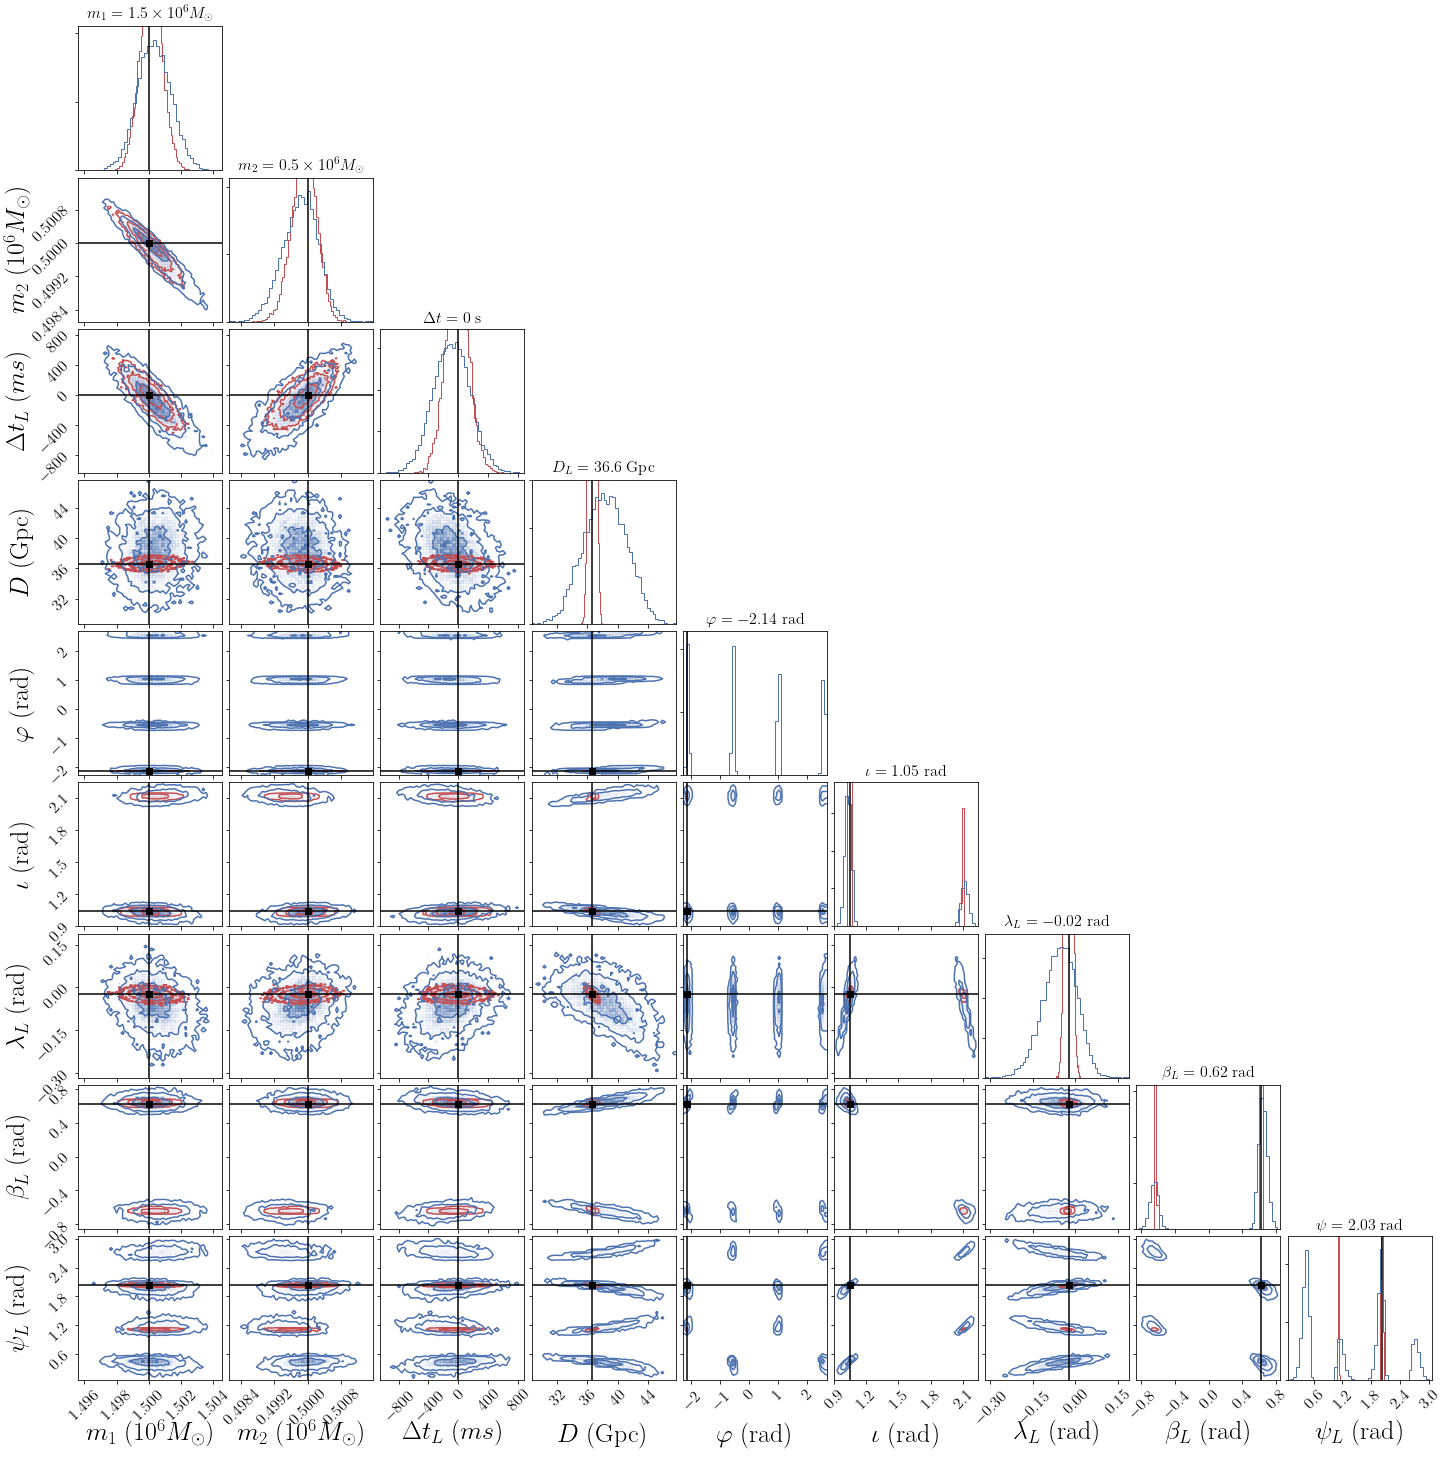
\includegraphics[width=.98\linewidth]{../plots/corner_smbh_case0_ptmcmc_22_hm.png}
  \caption{.}
  \label{fig:PEsmbh22hmCase0}
\end{figure*}

-- High-mass system, non-degenerate, 22 and HM + Fisher - stacked SNR contours
eg:

Case 12?
m1,    m2,    t0,D,     phi0,i,   lam,  bet, psi
8.89e5,1.11e5,0, 3.67e4,pi/3,pi/2,3pi/4,pi/3,pi/3

Case 0

-- Performance: waveform and likelihood costs, number of sampler evaluations

%%%%%%%%%%%%%%%%%%%%%%%%%%%%%%%%%%%%

\subsection{Accumulating signal with time}
\label{sec:SMBHPEacctime}

%%%%%%%%%%%%%%%%%%%%%%%%%%%%%%%%%%%%

\subsection{SNR dependence of parameter estimation}
\label{sec:SMBHPEdistance}

-- Move to Appendix ?

%%%%%%%%%%%%%%%%%%%%%%%%%%%%%%%%%%%%

\subsection{Highlighting degeneracies}
\label{sec:SMBHPEdegen}

\begin{figure*}
  \centering
  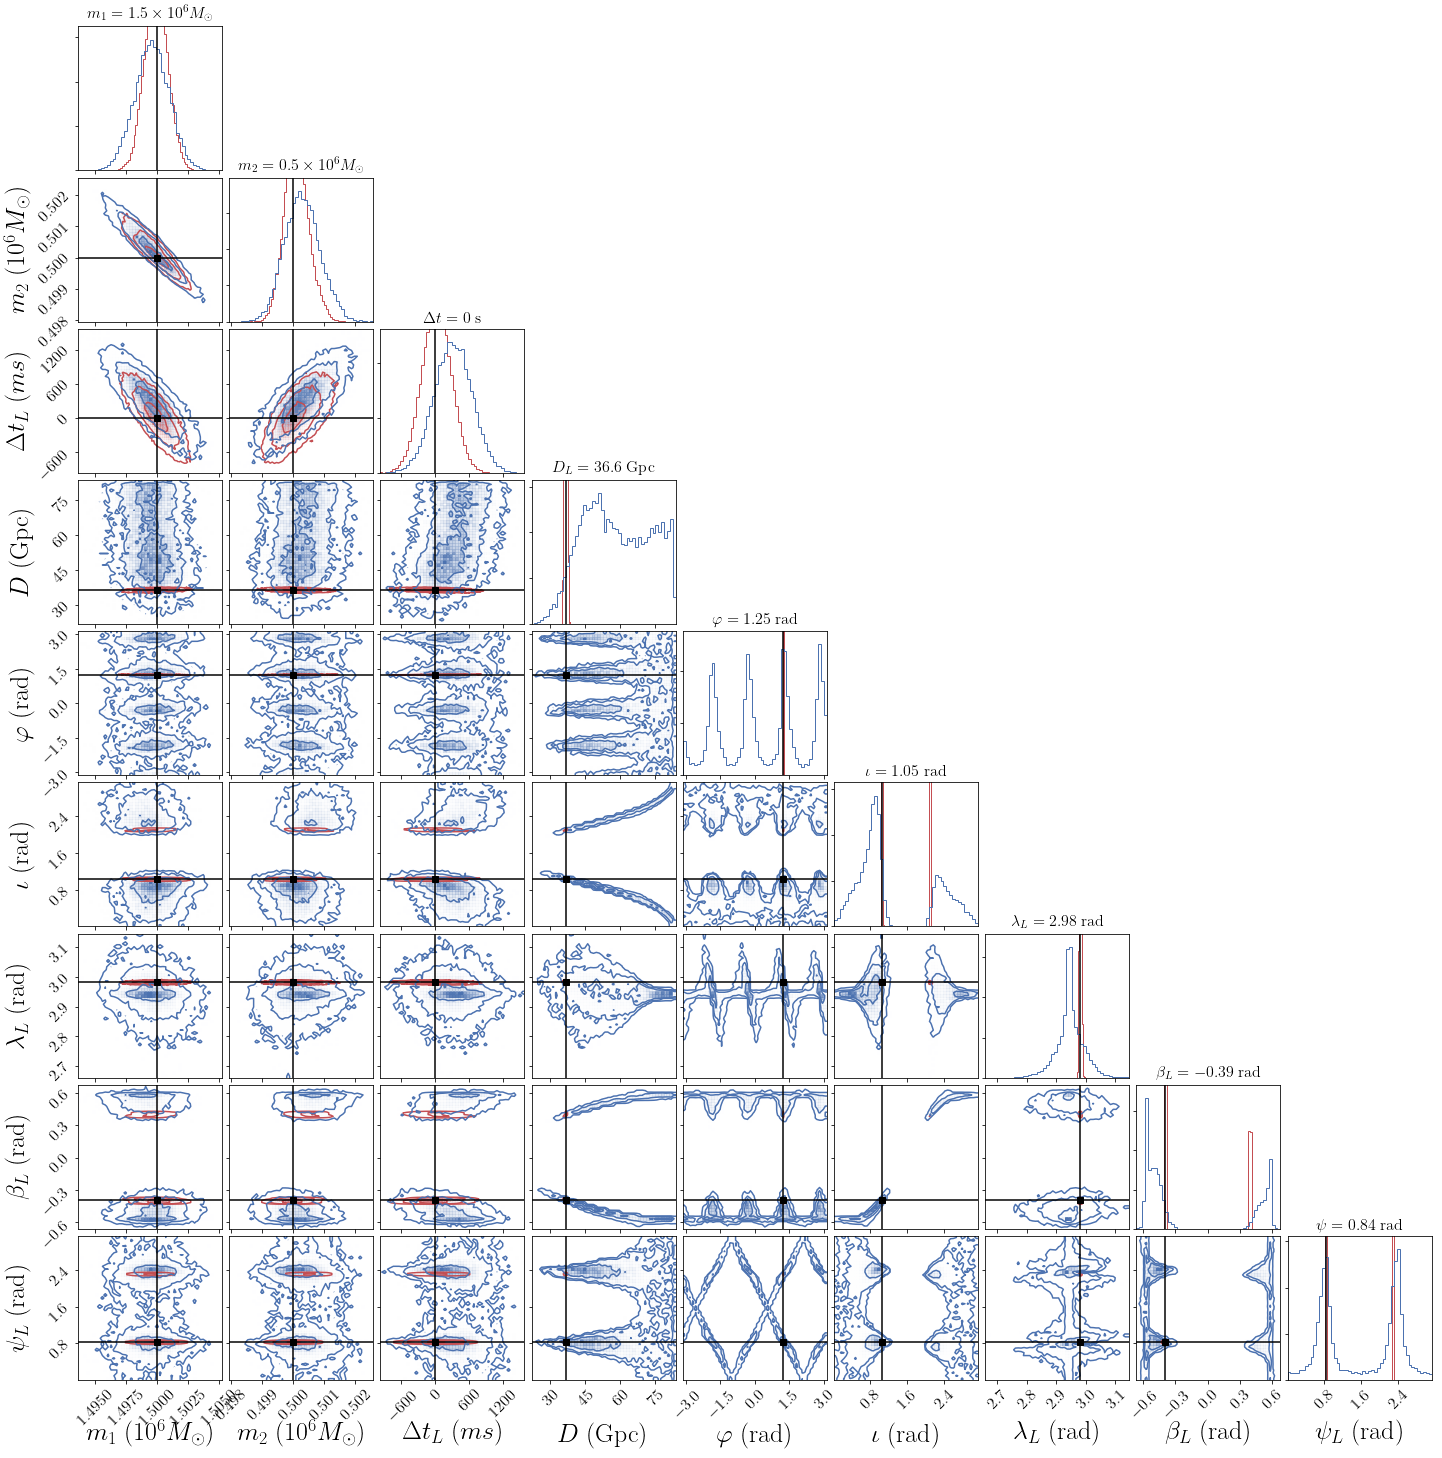
\includegraphics[width=.98\linewidth]{../plots/corner_smbh_case9_ptmcmc_22_hm.png}
  \caption{.}
  \label{fig:PEsmbh22hmCase0}
\end{figure*}

- Highlighting degeneracies

-- High-mass degenerate example, 22 vs HM - stacked SNR contours
-- show degenerate waveforms
-- simplified response and closed-form likelihood, full degeneracies
-- (explore simplified response further: parameter maps, other off-the-shelf samplers ?)

We can now explore possible degeneracies in the likelihood given by~\eqref{eq:simplelikelihood}, \eqref{eq:defsase} and \eqref{eq:defa22a2m2}-\eqref{eq:defe22e2m2}. We note that the relative contributions of the modes $h_{2,2}$ and $h_{2,-2}$ are strongly separated in the face-on or face-off limit, leading to a simplification of the response and an enhanced degeneracy. Due to the symmetry~\eqref{eq:symmetryresponse}, we will focus on the face-on limit $\iota \rightarrow 0$. In this limit, the $h_{2,-2}$ contributions die off rapidly as $a_{2,-2}\,, e_{2,-2} \sim \sin^{4} (\iota/2)$. If they are assumed to be negligible, then we can rewrite
\bsub\label{eq:saseapprox}
\begin{align}
	s_{a} \simeq i\calA e^{2 i \xi} \left( D_{a}^{+} + i D_{a}^{\times} \right) \,, \\
	s_{e} \simeq i\calA e^{2 i \xi} \left( D_{e}^{+} + i D_{e}^{\times} \right) \,,
\end{align}
\esub
where we introduced the notations $\xi (\varphiL, \psiL) \equiv -\varphiL - \psiL$ and $\calA(d, \iota) \equiv 3/4\sqrt{5/\pi}\cos^{4}(\iota/2)/d $ for the common phase and amplitude factors.

For a degeneracy to occur, both complex quantities $s_{a}$ and $s_{e}$ must be close to the injection values $s_{a}^{\rm inj}$ and $s_{e}^{\rm inj}$, which can be achieved as follows if~\eqref{eq:saseapprox} is valid. Defining the complex ratio
\be\label{eq:defr}
	r(\lambdaL, \betaL) = \frac{D_{a}^{+} + i D_{a}^{\times}}{D_{e}^{+} + i D_{e}^{\times} } \,,
\ee
if the position in the sky $(\lambda_{L}^{*}, \beta_{L}^{*})$ can be chosen so that
\be\label{eq:rcondition}
	r(\lambda_{L}^{*}, \beta_{L}^{*}) = \frac{s_{a}^{\rm inj}}{s_{e}^{\rm inj}} \,,
\ee
then adjusting $\calA$ and $\xi$ so that
\be
	i\calA e^{2 i \xi} = \frac{s_{a}^{\rm inj}}{\left( D_{a}^{+} + i D_{a}^{\times} \right)(\lambda_{L}^{*}, \beta_{L}^{*})}
\ee
generates degenerate points in parameter space with $\ln \calL \simeq 0$.

The conditions~\eqref{eq:defr}-\eqref{eq:rcondition} can be inverted for the sky position as follows. For a given complex value of $r = s_{a}^{\rm inj} / s_{e}^{\rm inj}$, $r(\lambda_{L}^{*}, \beta_{L}^{*}) = r$ can be rewritten as
\be\label{eq:eqtosolveforlambdabetaL}
	e^{4i\lambda_{L}^{*}}e^{i\frac{\pi}{3}} \frac{\left( 1 +\sin\beta_{L}^{*} \right)^{2}}{\left( 1 - \sin\beta_{L}^{*} \right)^{2}} = \frac{1+ i r}{1 - i r} \,.
\ee
Solving for the modulus of~\eqref{eq:eqtosolveforlambdabetaL} then yields
\be\label{eq:solutionbetaL}
	\sin\beta_{L}^{*} = \frac{\rho - 1}{\rho + 1} \,,
\ee
for
\be
	\rho = \sqrt{\left| \frac{1+ i r}{1 - i r} \right|} \,.
\ee
Solving for the argument of~\eqref{eq:eqtosolveforlambdabetaL} gives four solutions for $\lambda_{L}^{*}$ as
\be\label{eq:solutionlambdaL}
	\lambda_{L}^{*} = - \frac{\pi}{12} + \frac{1}{4}\mathrm{Arg} \frac{1+ i r}{1 - i r} + \frac{k \pi}{2} \quad \mathrm{for} \quad k = 0,\dots,3 \,.
\ee

Repeating the argument for the other branch of solutions $\iota \rightarrow \pi$ (or directly considering the symmery~\eqref{eq:symmetryresponse}) gives four other solutions in the sky with identical sky longitudes $\lambda_{L}^{*}$, with symmetrized sky latitudes $\beta_{L}^{*} \rightarrow -\beta_{L}^{*}$, and with $\xi (\varphiL, \psiL) \equiv -\varphiL + \psiL$, $\calA(d, \iota) \equiv 3/4\sqrt{5/\pi}\sin^{4}(\iota/2)/d $.

Thus, with~\eqref{eq:solutionbetaL}, \eqref{eq:solutionlambdaL} and $\beta_{L}^{*} \rightarrow -\beta_{L}^{*}$, we arrive at eight degenerate positions in the sky $(\lambda_{L}^{*}, \beta_{L}^{*})$. For each of these sky positions, an exact line degeneracy exists between $\varphiL$ and $\psiL$ as long as $\xi = \mathrm{const}$, as well as an approximate line degeneracy between $d$ and $\iota$, as long as $\calA = \mathrm{const}$, limited to inclination values where $\sin^{4}(\iota/2)$ (or $\cos^{4}(\iota/2)$, for the other branch of solutions) remains negligible. The combination of these degeneracies generates an extended structure in the multi-dimensional parameter space. As a result, when considering the marginal posterior for the sky position, these degenerate spots in the sky can have a lot of probability support.

%%%%%%%%%%%%%%%%%%%%%%%%%%%%%%%%%%%%
%%%%%%%%%%%%%%%%%%%%%%%%%%%%%%%%%%%%

\section{Stellar origin black holes}
\label{sec:SOBH}

-- SOBH system, SNR sufficient for clean analysis + Fisher - stacked SNR contours
-- Performance: waveform and likelihood costs, number of sampler evaluations

Stellar-origin black-hole (SOBH) mergers have been recently recognized as an
important source of LISA detections \cite{Sesana16} although full parameter
estimation studies are not available yet. In this section we present
three case studies of parameter inference for such sources. The parameters of
the simulated mergers are taken from the Radler LISA data challenge and are
listed in Table \ref{table:sobh_params}.
\begin{table}
	\begin{tabular}{|c||c|c|c|}
		\hline
		Radler entry 		& 1 	& 12 	& 52 \\
		\hline
		Mass 1 ($\Msol$) 	& 21.4	& 63.5	& 57.0 \\
		\hline
		Mass 2 ($\Msol$) 	& 20.1	& 45.1	& 36.8 \\
		\hline
		Distance (Mpc) 		& 49.1	& 318	& 308 \\
		\hline
		LISA SNR 			& 26.6	& 11.9	& 16.0 \\
		\hline
	\end{tabular}
	\caption{Parameters of the simulated SOBH mergers. \tdc{Maybe we can show
			 these on the upper right of each corner plot instead.}}
	\label{table:sobh_params}
\end{table}

The waveform model used to work with such systems is the phenomenological
approximant IMRPhenomD, extended at low frequency with a post-Newtonian
frequency-domain waveform. In practice, because LISA only observes the early
inspiral of SOBH systems, only the post-Newtonian waveform plays a role here.
We do not expect radiation modes beyond the quadrupole to give a significant
contribution to the parameter estimates, so we only include the $(2,2)$ mode
for simplicity. We do not include any effect arising from black-hole spins.

As done in the previous section, we apply our parameter inference procedure to
these systems using both BAMBI and parallel-tempered MCMC sampling, and we
numerically evaluate the Fisher matrix at the parameters of the injection.

Due to the duration of an SOBH inspiral in the LISA band, and the complete lack
of merger and ringdown, the chirp mass $\Mchirp$ is measured much better than
other mass parameters and the component masses have a much stronger correlation
than usually found with ground-based gravitational-wave detectors. In order for
the sampling to converge robustly in a reasonable time, we find it is necessary
to express the mass parameters in terms of $\Mchirp$ and symmetric mass ratio
$\eta$, and a relatively tight prior around the injected parameters is required
as well.

In order to generate these results, our PTMCMC sampler requires between
$5\times 10^5$ and $3\times 10^6$ steps with 100 temperatures, taking on the
order of days on a single CPU core without careful optimization. The BAMBI
sampling, on the other hand, completes in tens of minutes only.

The resulting posterior distributions are shown in Fig.~\ref{fig:sobh_corner_1}
and \ref{fig:sobh_corner_12}. We find close agreement between the BAMBI and
PTMCMC samplers. The full joint distributions are fairly complex, but the
complexity is mostly restricted to multimodalities and degeneracies in the
angular parameters only. The typical degeneracy between inclination and distance
is evident. Masses, merger time, distance, inclination and sky location, which
are arguably the most astrophysically useful parameters, have simple marginal
distributions with a well-defined mode and close to Gaussian, even at these
moderate SNR values. The Fisher matrix estimates represent the marginal
distributions of these parameters at least to the order of magnitude. In some
cases the Fisher estimates approximate very precisely even the joint
distributions of pairs of these parameters.

\begin{figure*}
	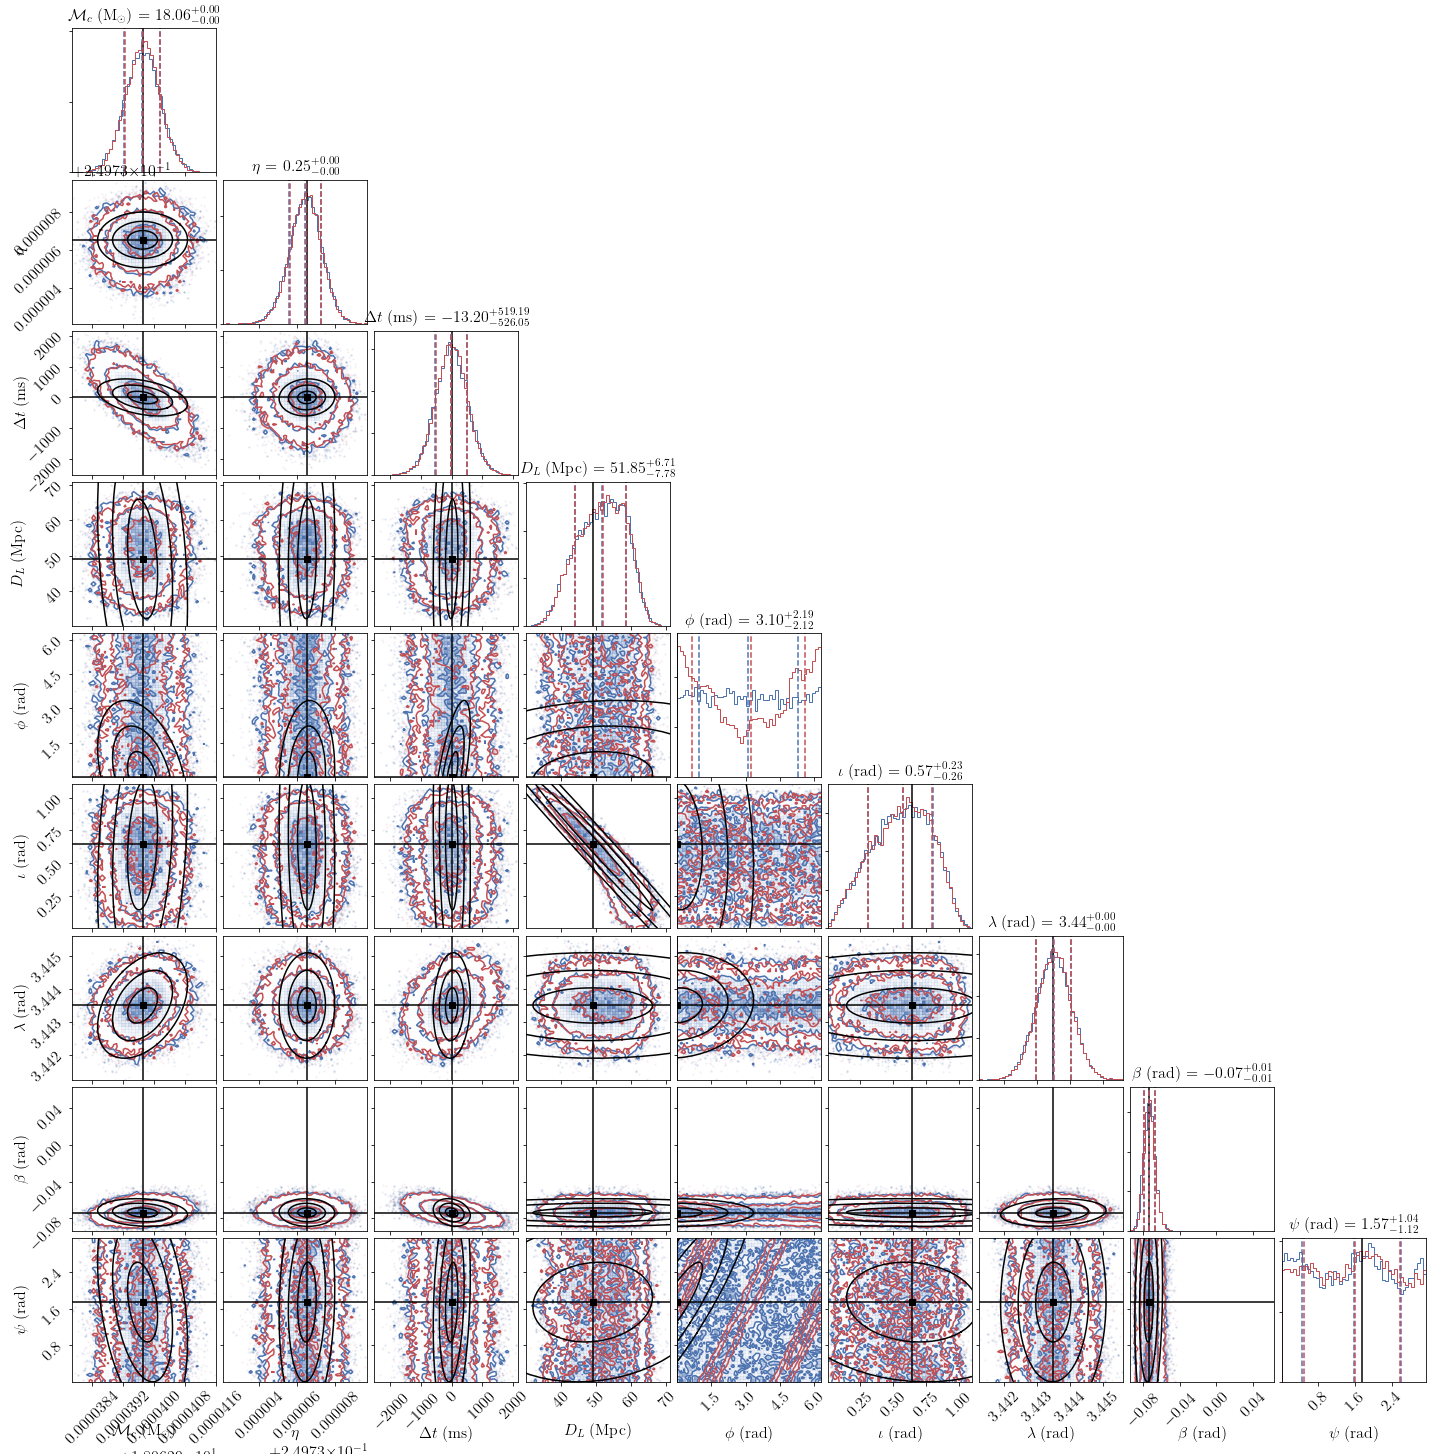
\includegraphics[width=\textwidth]{../plots/corner_sobh_tdc1_ptmcmc_bambi}
	\caption{Inferred parameter posterior distribution for SOBH system 1.}
	\label{fig:sobh_corner_1}
\end{figure*}

\begin{figure*}
	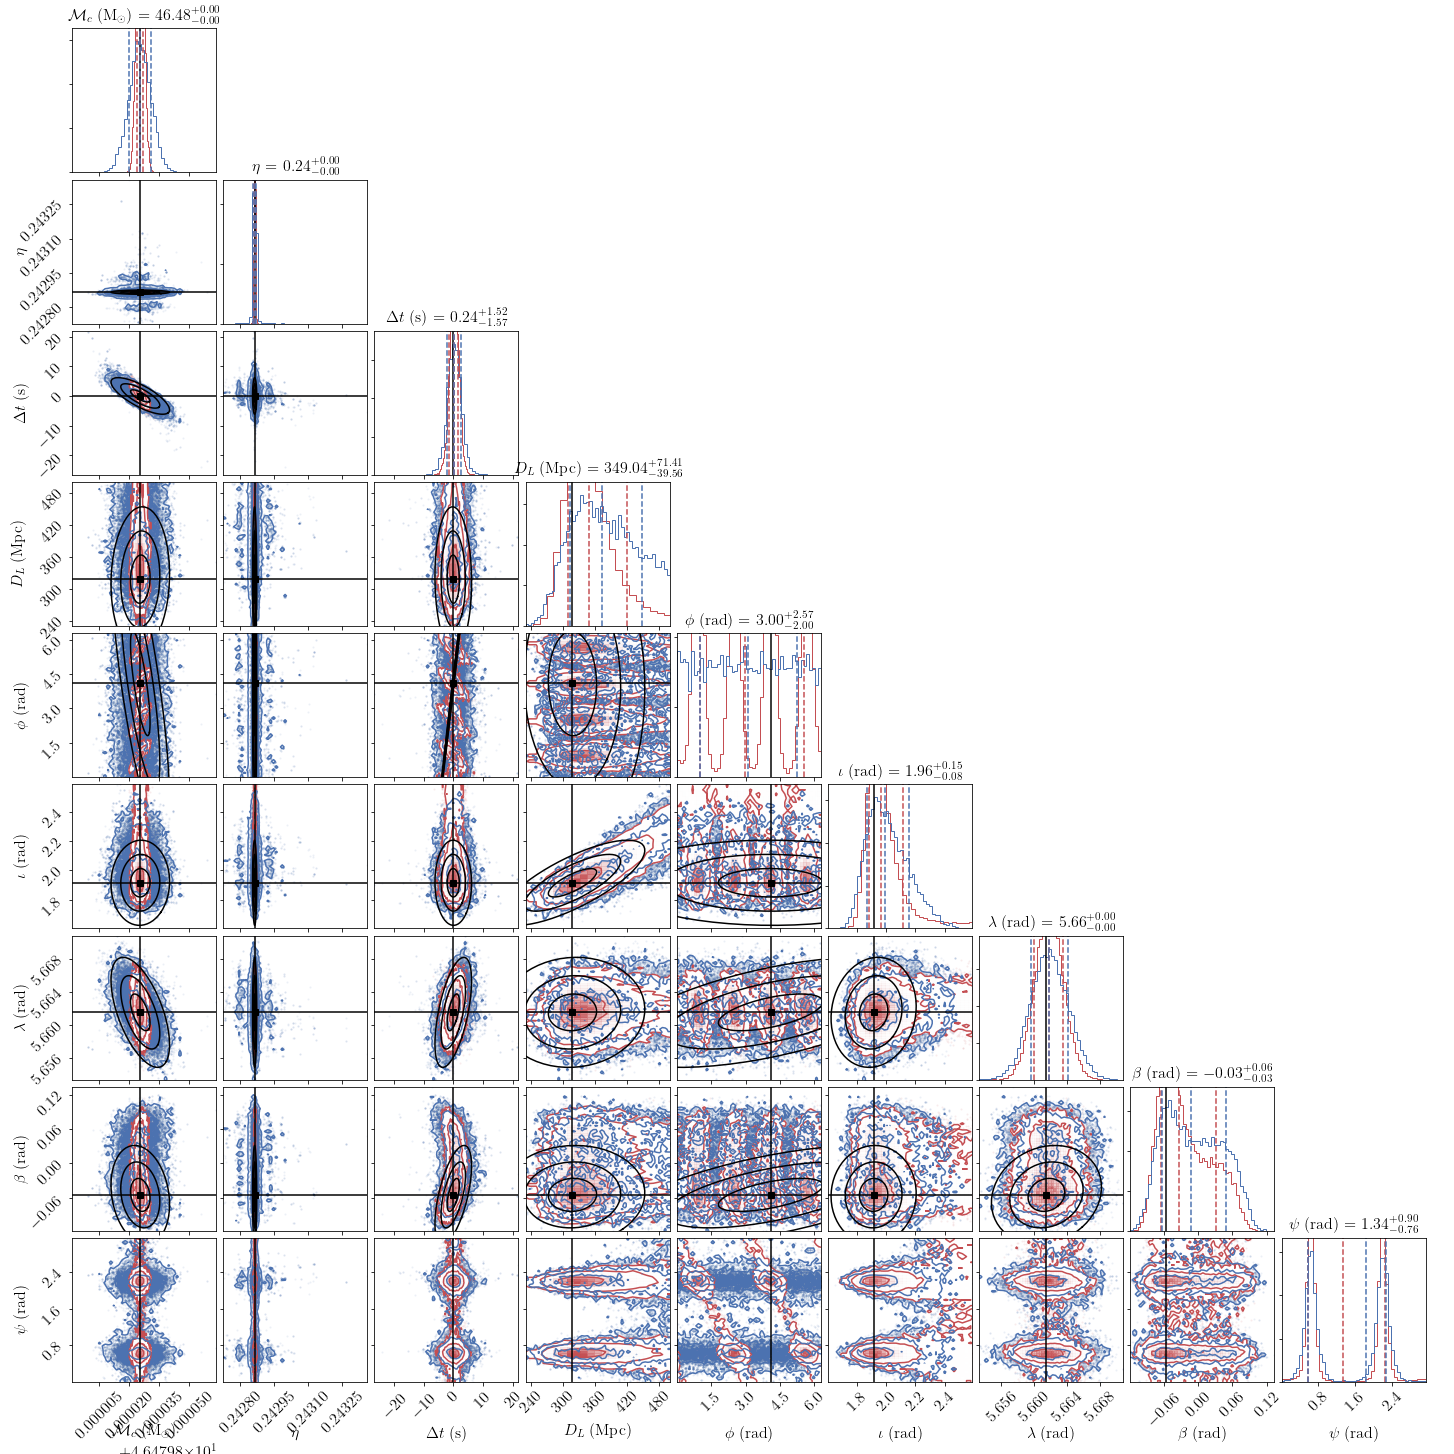
\includegraphics[width=\textwidth]{../plots/corner_sobh_tdc2_ptmcmc_bambi}
	\caption{Inferred parameter posterior distribution for SOBH system 12.}
	\label{fig:sobh_corner_12}
\end{figure*}

%%%%%%%%%%%%%%%%%%%%%%%%%%%%%%%%%%%%
%%%%%%%%%%%%%%%%%%%%%%%%%%%%%%%%%%%%

\section{Discussion}
\label{sec:discussion}

- Summary/conclusions


----------------
Other questions:
- special orientations/sky locations ?
- Fisher matrix qualification - explore parameter choices
- continuously increase SNR - include on these examples
- continuously accumulate information over time
- full exploration of parameter space for all of the above...


%%%%%%%%%%%%%%%%%%%%%%%%%%%%%%%%%%%%
%%%%%%%%%%%%%%%%%%%%%%%%%%%%%%%%%%%%

\appendix

%%%%%%%%%%%%%%%%%%%%%%%%%%%%%%%%%%%%
%%%%%%%%%%%%%%%%%%%%%%%%%%%%%%%%%%%%

\section{Numerical integration with spline-interpolated phases}
\label{sec:numintegration}

[describe implementation of 0-noise integrals]

%%%%%%%%%%%%%%%%%%%%%%%%%%%%%%%%%%%%
%%%%%%%%%%%%%%%%%%%%%%%%%%%%%%%%%%%%

\section{Reduced-order model for EOBNRv2HMROM}
\label{sec:rom}

[describe implementation of the ROM]

%%%%%%%%%%%%%%%%%%%%%%%%%%%%%%%%%%%%
%%%%%%%%%%%%%%%%%%%%%%%%%%%%%%%%%%%%

\bibliography{references.bib}

\end{document}
